%%% The main file. It contains definitions of basic parameters and includes all other parts.

%% Settings for single-side (simplex) printing
% Margins: left 40mm, right 25mm, top and bottom 25mm
% (but beware, LaTeX adds 1in implicitly)
\documentclass[12pt,a4paper]{report}
\setlength\textwidth{145mm}
\setlength\textheight{247mm}
\setlength\oddsidemargin{15mm}
\setlength\evensidemargin{15mm}
\setlength\topmargin{0mm}
\setlength\headsep{0mm}
\setlength\headheight{0mm}
% \openright makes the following text appear on a right-hand page
\let\openright=\clearpage

%% Settings for two-sided (duplex) printing
% \documentclass[12pt,a4paper,twoside,openright]{report}
% \setlength\textwidth{145mm}
% \setlength\textheight{247mm}
% \setlength\oddsidemargin{14.2mm}
% \setlength\evensidemargin{0mm}
% \setlength\topmargin{0mm}
% \setlength\headsep{0mm}
% \setlength\headheight{0mm}
% \let\openright=\cleardoublepage

%% Character encoding: usually latin2, cp1250 or utf8:
\usepackage[utf8]{inputenc}

%% Further useful packages (included in most LaTeX distributions)
\usepackage{amsmath}        % extensions for typesetting of math
\usepackage{amsfonts}       % math fonts
\usepackage{amsthm}         % theorems, definitions, etc.
\usepackage{bbding}         % various symbols (squares, asterisks, scissors, ...)
\usepackage{bm}             % boldface symbols (\bm)
\usepackage{graphicx}       % embedding of pictures
\usepackage{fancyvrb}       % improved verbatim environment
\usepackage{natbib}         % citation style AUTHOR (YEAR), or AUTHOR [NUMBER]
\usepackage[nottoc]{tocbibind} % makes sure that bibliography and the lists
			    % of figures/tables are included in the table
			    % of contents
\usepackage{dcolumn}        % improved alignment of table columns
\usepackage{booktabs}       % improved horizontal lines in tables
\usepackage{paralist}       % improved enumerate and itemize
\usepackage[table]{xcolor}  % typesetting in color


\PassOptionsToPackage{hyphens}{url}

%%% Basic information on the thesis

% Thesis title in English (exactly as in the formal assignment)
\def\ThesisTitle{Comparison of Approaches for Querying of Chemical Compounds}

% Author of the thesis
\def\ThesisAuthor{Bc. Vojtěch Šípek}

% Year when the thesis is submitted
\def\YearSubmitted{2017}

% Name of the department or institute, where the work was officially assigned
% (according to the Organizational Structure of MFF UK in English,
% or a full name of a department outside MFF)
\def\Department{Department of Software Engineering}

% Is it a department (katedra), or an institute (ústav)?
\def\DeptType{Department}

% Thesis supervisor: name, surname and titles
\def\Supervisor{doc. RNDr. Irena Holubová, Ph.D.}

% Supervisor's department (again according to Organizational structure of MFF)
\def\SupervisorsDepartment{Department of Software Engineering}

% Study programme and specialization
\def\StudyProgramme{Computer Science}
\def\StudyBranch{Software Systems}

% An optional dedication: you can thank whomever you wish (your supervisor,
% consultant, a person who lent the software, etc.)
\def\Dedication{%
Dedication.
}

% Abstract (recommended length around 80-200 words; this is not a copy of your thesis assignment!)
\def\Abstract{%
Abstract.
}

% 3 to 5 keywords (recommended), each enclosed in curly braces
\def\Keywords{%
{key} {words}
}

%% The hyperref package for clickable links in PDF and also for storing
%% metadata to PDF (including the table of contents).
\usepackage[pdftex,unicode]{hyperref}   % Must follow all other packages
\hypersetup{breaklinks=true}
\hypersetup{pdftitle={\ThesisTitle}}
\hypersetup{pdfauthor={\ThesisAuthor}}
\hypersetup{pdfkeywords=\Keywords}
\hypersetup{urlcolor=blue}

% Definitions of macros (see description inside)
%%% This file contains definitions of various useful macros and environments %%%
%%% Please add more macros here instead of cluttering other files with them. %%%

%%% Minor tweaks of style

% These macros employ a little dirty trick to convince LaTeX to typeset
% chapter headings sanely, without lots of empty space above them.
% Feel free to ignore.
\makeatletter
\def\@makechapterhead#1{
  {\parindent \z@ \raggedright \normalfont
   \Huge\bfseries \thechapter. #1
   \par\nobreak
   \vskip 20\p@
}}
\def\@makeschapterhead#1{
  {\parindent \z@ \raggedright \normalfont
   \Huge\bfseries #1
   \par\nobreak
   \vskip 20\p@
}}
\makeatother

% This macro defines a chapter, which is not numbered, but is included
% in the table of contents.
\def\chapwithtoc#1{
\chapter*{#1}
\addcontentsline{toc}{chapter}{#1}
}

% Draw black "slugs" whenever a line overflows, so that we can spot it easily.
\overfullrule=1mm

%%% Macros for definitions, theorems, claims, examples, ... (requires amsthm package)

\theoremstyle{plain}
\newtheorem{thm}{Theorem}
\newtheorem{lemma}[thm]{Lemma}
\newtheorem{claim}[thm]{Claim}

\theoremstyle{plain}
\newtheorem{defn}{Definition}

\theoremstyle{remark}
\newtheorem*{cor}{Corollary}
\newtheorem*{rem}{Remark}
\newtheorem*{example}{Example}

%%% An environment for proofs

%%% FIXME %%% \newenvironment{proof}{
%%% FIXME %%%   \par\medskip\noindent
%%% FIXME %%%   \textit{Proof}.
%%% FIXME %%% }{
%%% FIXME %%% \newline
%%% FIXME %%% \rightline{$\square$}  % or \SquareCastShadowBottomRight from bbding package
%%% FIXME %%% }

%%% An environment for typesetting of program code and input/output
%%% of programs. (Requires the fancyvrb package -- fancy verbatim.)

\DefineVerbatimEnvironment{code}{Verbatim}{fontsize=\small, frame=single}

%%% The field of all real and natural numbers
\newcommand{\R}{\mathbb{R}}
\newcommand{\N}{\mathbb{N}}

%%% Useful operators for statistics and probability
\DeclareMathOperator{\pr}{\textsf{P}}
\DeclareMathOperator{\E}{\textsf{E}\,}
\DeclareMathOperator{\var}{\textrm{var}}
\DeclareMathOperator{\sd}{\textrm{sd}}

%%% Transposition of a vector/matrix
\newcommand{\T}[1]{#1^\top}

%%% Various math goodies
\newcommand{\goto}{\rightarrow}
\newcommand{\gotop}{\stackrel{P}{\longrightarrow}}
\newcommand{\maon}[1]{o(n^{#1})}
\newcommand{\abs}[1]{\left|{#1}\right|}
\newcommand{\dint}{\int_0^\tau\!\!\int_0^\tau}
\newcommand{\isqr}[1]{\frac{1}{\sqrt{#1}}}

%%% Various table goodies
\newcommand{\pulrad}[1]{\raisebox{1.5ex}[0pt]{#1}}
\newcommand{\mc}[1]{\multicolumn{1}{c}{#1}}


% Title page and various mandatory informational pages
\begin{document}
%%% Title page of the thesis and other mandatory pages

%%% Title page of the thesis

\pagestyle{empty}
\hypersetup{pageanchor=false}
\begin{center}

\centerline{\mbox{
\includegraphics[width=166mm]{../img/logo-en.pdf}}}

\vspace{-8mm}
\vfill

{\bf\Large MASTER THESIS}

\vfill

{\LARGE\ThesisAuthor}

\vspace{15mm}

{\LARGE\bfseries\ThesisTitle}

\vfill

\Department

\vfill

\begin{tabular}{rl}

Supervisor of the master thesis: & \Supervisor \\
\noalign{\vspace{2mm}}
Study programme: & \StudyProgramme \\
\noalign{\vspace{2mm}}
Study branch: & \StudyBranch \\
\end{tabular}

\vfill

% Zde doplňte rok
Prague \YearSubmitted

\end{center}

\newpage

%%% Here should be a bound sheet included -- a signed copy of the "master
%%% thesis assignment". This assignment is NOT a part of the electronic
%%% version of the thesis. DO NOT SCAN.

%%% A page with a solemn declaration to the master thesis

\openright
\hypersetup{pageanchor=true}
\pagestyle{plain}
\pagenumbering{roman}
\vglue 0pt plus 1fill

\noindent
I declare that I carried out this master thesis independently, and only with the cited
sources, literature and other professional sources.

\medskip\noindent
I understand that my work relates to the rights and obligations under the Act No.~121/2000 Sb.,
the Copyright Act, as amended, in particular the fact that the Charles
University has the right to conclude a license agreement on the use of this
work as a school work pursuant to Section 60 subsection 1 of the Copyright Act.

\vspace{10mm}

\hbox{\hbox to 0.5\hsize{%
In ........ date ............	% FIXME!
\hss}\hbox to 0.5\hsize{%
signature of the author
\hss}}

\vspace{20mm}
\newpage

%%% Mandatory information page of the thesis

\openright

\vbox to 0.5\vsize{
\setlength\parindent{0mm}
\setlength\parskip{5mm}

Title:
\ThesisTitle

Author:
\ThesisAuthor

\DeptType:
\Department

Supervisor:
\Supervisor, \SupervisorsDepartment

Abstract:
\Abstract

Keywords:
\Keywords

\vss}

\newpage

%%% Dedication

\openright

\noindent
\Dedication

\newpage

\openright
\pagestyle{plain}
\pagenumbering{arabic}
\setcounter{page}{1}


%%% A page with automatically generated table of contents of the master thesis

\tableofcontents

%%% Each chapter is kept in a separate file
\chapter*{Introduction}
\addcontentsline{toc}{chapter}{Introduction}

Querying is the essential utility of each database and the same applies to chemical databases. Nowadays, the largest publicly accessible databases contain around 100 million compounds. The chemical compounds can be naturally represented as graphs where atoms are represented as vertices and bonds are represented as edges. The typical chemical compound is a connected sparse graph with labeled edges and vertices where the size of the labeling alphabet for edges is less than 10 and size of the labeling alphabet for vertices is in order of low hundreds.\\

The size of chemical compounds is variable. The vertex count varies typically from very small compounds with less then 10 vertices to huge compounds with hundreds of vertices. These sizes multiplied by the size of the database implies that the querying over such databases might be challenging task.\\

The most common queries over chemical databases are exact match query, shortest path search, similarity search and substructure search which are usually used in graph databases. The latter will be the main point of interest in this thesis.\\

The goal of subgraph querying is to obtain a list of graphs from the database which contain the queried graph as its subgraph. The result of this process has a wide range of utilization e.g. in chemoinformatics and bioinformatics and therefore in pharmaceutic industry. Since it is known as NP-complete problem several indexing techniques has been proposed to minimize the count of subgraph isomorphism tests.\\

There are several benchmarks of the mentioned indexing techniques already. The problem is that all found benchmarks has been created by the authors of some of the indexing technique and therefore the intention of the benchmark is to show that the particular index is more powerful than others. There is a lack of independent benchmarks which would compare the best performing indexes on the same data and on the same hardware.\\  

In this thesis we compare the best performing indexing techniques using the same environment. We also compare these techniques with the classical SQL database performance as well as with the performance of the modern graph databases.


\section*{Structure of the Thesis}
\addcontentsline{toc}{section}{Structure of the Thesis}

This thesis is divided into four main parts. In the first part called \textit{Base Terms and Definitions} we define the main problem of this thesis, subgraph isomorphism, and we define the main terms related to the graph theory which are used later in the thesis.

In the second part called \textit{Analysis of Related Work} we analyze the found literature about the algorithms for resolving subgraph isomorphism problem and most importantly we analyze and briefly describe the indexing techniques proposed in related work.\\

In the third part, \textit{Experimental Work}, several hypotheses are formulated. For their verification the author’s experimental work is used. These experiments are described in detail and the issues found out during the implementation are explored.\\

The last part of the thesis called \textit{Experimental Results} covers the results of experimental work and the comparison with results of related researches. We will comment on the findings and propose some directions in possible following research.

\chapter{Analysis of Related Work}

In this chapter we summarize the work done by other authors which is related to the topic of this thesis. At first we summarize the algorithms which have been developed for subgraph isomorphism matching and their comparison. Next we describe indices which might be used for obtaining the candidate set and algorithms which are used for their construction. The part of this chapter focuses on approaches which utilize query mechanisms of particular relational and graph databases. In the last part we provide a summary of commercially used solutions.\\

As stated before the typical workflow in subgraph querying process has two parts:

\begin{itemize}
	\item \textbf{Candidate set creation} - on the basis of a pre-built index the whole \linebreak database is pruned to obtain as small set of graphs as possible which contains all records which satisfy the specified query.
	
	\item \textbf{Verification} - the process of isolating false positives from the candidate set. In this phase the algorithm for subgraph isomorphism recognition has to be used.
	
\end{itemize}

Since subgraph isomorphism problem is NP-complete, we cannot expect significant improvement in the verification phase which implies that good pruning of database is essential for effective subgraph querying.



\section{Subgraph Isomorphism Algorithms Survey}

This section does not provide in-depth comparison of available algorithms since it is not a main topic of this thesis.\\

Almost all papers related to subgraph query methods refer two algorithms - Ullmann\cite{Ullmann} and VF2\cite{VF2}. Those two algorithms are deeply compared in the \cite{Ehrlich2012} benchmark where VF2 outperforms the Ullmann.\\

In \cite{Lee} there is a comparison of four algorithms derived from Ullmann algorithm. These are VF2, QuickSI \cite{QuickSI}, GraphQL \cite{GraphQL}, GADDI \cite{GADDI} and SPath \cite{SPath}. They were compared on three real-world data sets. Although all three comparisons have a different winner, it seems that the most efficient algorithm is QuickSI in an average use-case.

\section{Comparison and Summary of Index Building Methods}

In the first part of this section we briefly describe algorithms for building indices on top of chemical compound databases. These are \textit{GraphGrep} \cite{GraphGrep}\cite{GrahGrep:intro}, \textit{GIndex} \cite{GIndex}, \textit{GString} \cite{GString}, \textit{GraphGrepSX} \cite{GraphGrepSX}, \textit{GIRAS} \cite{GIRAS}, \textit{C-tree} \cite{CTree} and \textit{GDIndex} \cite{GDIndex}\\

They form just a selection from a much bigger set of applicable methods and they were picked for different reasons:

\begin{itemize}
	\item The method is mentioned in a majority of relevant articles
	\item The method uses an original algorithm or data structure
	\item The method has excellent results in benchmarks
\end{itemize}

Some of them can be used in generic graph databases, some of them are very specific to the field of chemical compounds but with some effort they might be used also for other graph databases with specific point of interest.

In the following sections we will briefly introduce the basic ideas behind all the previously mentioned methods.

\subsection{GraphGrep}

Very simple and intuitive indexing technique which can be used in any graph database with labeled graphs is called \textit{GraphGrep}. The presumption is that every vertex has a defined unique ID.\\

For each graph in the database there is constructed index represented as a hash table where the key is a hashed value of a \textit{label-path} (a concatenation of the vertex/edge labels on the path) and the value is a number of unique \textit{id-paths} (a concatenation of the vertex IDs on the path) which represent a particular \textit{label-path} in the graph. In the hash table there are all \textit{label-paths} which are present in the graph up to length \textit{l} where \textit{l} is a parameter. This hash table is called a \textit{graph fingerprint}.\\

For example the graph in Figure~\ref{fig:graphgrep} would be represented in the index with $l=3$ as depicted in Table \ref{tab:graphgrep}. The numbers on the picture represent the vertex ID, characters next the each vertex represent its label.

\begin{figure}[h]
	\centering
	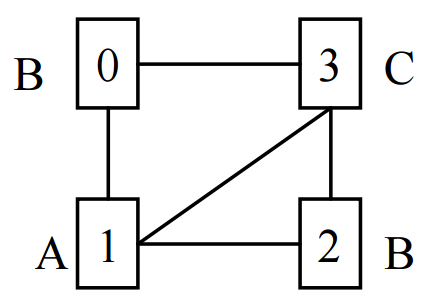
\includegraphics[width=0.25\textwidth]{../img/graphgrep.png}
	\caption{GraphGrep example graph}
	\label{fig:graphgrep}
\end{figure}

\begin{table}[h]
	\centering
	\renewcommand{\arraystretch}{2.5}
	\setlength{\arrayrulewidth}{0.5mm
	}
	\begin{tabular}[h!]{|p{3cm} p{3cm}|p{3cm} p{3cm}|}
		\hline
		\rowcolor{lightgray}
		Key & Value & Key & Value\\ \hline
		h(A) & 1 & h(ABC) & 2\\
		h(B) & 2 & h(ACB) & 2\\
		h(C) & 1 & h(BAC) & 2\\
		h(AB) & 2 & h(BCA) & 2\\
		h(AC) & 1 & h(BAB) & 2\\
		h(BA) & 2 & h(BCB) & 2\\
		h(BC) & 2 & h(CBA) & 2\\
		h(CA) & 1 & h(CAB) & 2\\
		h(CB) & 2 & & \\ \hline
	\end{tabular}
\caption{GraphGrep example graph fingerprint}
\label{tab:graphgrep}
\end{table}

The same process is used for the query. The query itself is also a graph and therefore the hash table can be created too. Then, in the candidate set creation part, each graph’s fingerprint is compared to the query fingerprint.

If any value in the query fingerprint is higher than value in the graph fingerprint for the same key or when some key from the query fingerprint is missing in the graph's fingerprint, it means that this graph can be filtered out from the candidate set because we know that the query cannot be its subgraph.

\subsection{GIndex}

This method utilizes the concepts of \textit{frequent subgraphs} and \textit{discriminative fragments}. It also comes with an innovative data structure for storing the index.\\

Since the number of all subgraphs grows exponentially with the size of the graph and therefore it would be impossible to index all of them, we need to prune the number of index records to be as compact and still as efficient as possible.\\

Because of the mentioned reasons the \textit{frequent subgraphs} and \textit{discriminative fragments} concepts have a significant role.\\

\textbf{Frequent subgraphs} are all subgraphs which are contained in at least \linebreak $ minSup $ (minimum support) graphs in the database. The survey of frequent subgraphs mining can be found in \cite{frequentGraphs}. Suppose we have an index from all frequent subgraphs and for each record in the index we have a set of IDs of graphs in the database in which it occurs. If the query graph $ q $ is frequent, we have the candidate set immediately. If not, we can get the candidate set as an intersection of matched graphs sets of all frequent subgraphs of $ q $.\\

Utilization of pure set of frequent subgraphs with static $ minSup $ attribute has a couple of issues. With $ minSup $ set too low, we get an enormous set of frequent subgraphs. If the $ minSup $ is too high, the candidate set can be too large (at least $ minSup $) with larger probability of false positives.\\

That is why the described method comes with size-increasing support function. It is a non-decreasing function which takes the graph size as an argument (defined as the number of edges) and returns the $ minSup $ for given size. This results with smaller $ minSup $ for small graphs (because of the efficiency) and bigger $ minSup $ for large graphs (because of the compactness). It is necessary to have specified limit starting from which the function returns infinite to not have too big subgraphs in the index.\\


An additional pruning of the index can be done. There is a very high chance that frequent subgraph $ g $ will not be enough discriminative. It means that  the candidate set of $ g $ is not significantly smaller than the intersection of candidate sets of its subgraphs.\\

\textbf{Discriminative fragments} concept brings a new metric. It measures how much discriminative the frequent subgraph is comparing to the set of its subgraphs in the index. The discriminative ratio is defined as

$$ \gamma = \frac{|\bigcap _{i} D_{f_{\varphi i}} |}{| D_{x} |} $$

\noindent where $D_{x}$ is the set of graphs containing $ x $ and $ D_{f_{\varphi i}} $ is the set of graphs which contain subgraphs of $ x $ which are in the index. If the discriminative ratio is close to 1, we know that the discriminative power is low.\\

\textbf{gIndex} is a prefix tree data structure. Its nodes are of 2 types - \textit{discriminative} and \textit{redundant}. Each node’s key is a text string which represents the subgraph. It is serialized and canonized based on special application of DFS algorithm. This technique is called \textit{DFS Coding} and is described in \cite{gspan}.

Discriminative nodes are both frequent (based on given \textit{size-increasing support function}) and discriminative (based on specified $ \gamma $) and they contain a list of IDs of all graphs in the database which contain the particular subgraph. Redundant nodes are present just to satisfy the structure of the \textit{gIndex} tree.\\

The Root of the tree is an empty graph, whose candidate set is the whole database. Level 1 of the tree is the set of vertices (graphs of size 0). Each node in the tree (from level 2) has 1 more edge than its parent (because of the canonization it has its parent’s key as its prefix).\\

It would be very inefficient to check all subgraphs of a query graph. But, we know that if the subgraph $ g $ is not present in the graph $ G $ then no superstructure of $ g $ is present in $ G $. Also we know that if $ g $ and $ h $ are subgraphs of $ G $ and $ g \subset h $ then the candidate set generated by $ h $ is a subset of candidate set generated by $ g $ and therefore it has a bigger pruning power and usage of $ g $ is redundant.\\

From the two previously mentioned statements it is clear what is the search algorithm. We need to enumerate all fragments of the query graph $ q $ starting from 1-node fragments and iteratively enlarge the fragments by adding 1 edge each time. We stop this process at the point where the fragment is not in the index anymore.\\

Each of the fragments which were created in the last iteration can be found in the index. We only need to check whether the matched node in the index is discriminative or redundant. If it is redundant, we find the closest discriminative node on the path to root. Having the set of matched discriminative nodes in the tree, we compute an intersection of their sets of matched graphs in the database to get the desired candidate set.

\subsection{GString}

All other methods can be used in any graph database. On the other hand, GString method is very specific for the organic chemical databases (but can be internally modified to support different graph databases with specific content).\\

The main ideas come from the knowledge of common structures of the graphs in the database. The chemical compounds consist of 3 types of semantic structures - paths, cycles and stars (a central node with a fanout). Each chemical compound can be converted into a graph whose nodes are not atoms but one of the mentioned structures. This converted graph is significantly smaller than the original one.\\

The other observation is that we can omit the hydrogens since their number can be easily computed and we can omit the labels of carbon atoms and single (saturated) bonds.\\

Based on previous preliminaries, each graph in the database can be shrinked to the graph of common structures. Each node contains 3 types of information:

\begin{itemize}
	\item \textbf{Type} - path, cycle or star
	\item \textbf{Size} - For path and cycle it is the number of nodes, for star it is the fan-out
	
	\item \textbf{Triple} $ <n_{n}, n_{b}, n_{e}> $ where:
	\begin{itemize}
		\item $ n_{n} $ is the number of non-carbon atoms
		\item $ n_{b} $ is the number of branches (connected paths of the length 1)
		\item $ n_{e} $ is the number of double or triple bonds
	\end{itemize}
	
\end{itemize}

For each such graph we can get a set of all paths up to length $ l $. The index structure of GString method is a suffix tree of those paths, where each node is identified by tuple $ <Type, Size> $ and contains a set of pointers to the table where quadruples $ <n_{n}, n_{b}, n_{e}, id> $ are stored for matched nodes from a particular graph. The suffix tree is filled up by all paths up to length $ l $ from all graphs in the database.\\

The candidate set is obtained as follows. The query graph itself is translated to the common structure graph by the same process which was utilized for index building. Then we just identify suffix tree nodes which were visited and use the pointers to the detail table in such nodes. The graph is added into the candidate set if it is represented in each visited suffix tree node and if the triple $ <n_{n}, n_{b}, n_{e}> $ satisfies the query.

It means that for cycles, the $ n_{n} $ and $ n_{e} $ has to be equivalent in both query and database record, $n_{b}$ has to be equal or lower in the query comparing to the database record. For the paths and stars all three attributes has to be same or lower in the query.\\

Note that the answer set of this method can be different from previous methods. Let us take a path of four carbons $ c-c-c-c $ as an example of a query and assume that the benzene (cycle of six carbons) is a part of the database. The previous methods marks the benzene as a \textit{match}. On the other hand the GString will filter it out from the candidate set because it finds out that its \textit{common structure} graph is completely different.\\

However, this is a correct behavior for the chemical compound database since we can expect that if somebody asks for a path of four carbons, he or she does not expect a benzene as a result since cycles and paths have different semantics.

\subsection{GraphGrepSX}

GraphGrepSX is an improved version of GraphGrep. It uses the very same approach for obtaining all the indexed features - it takes all the paths up to the length $l$ from all the graphs in the database. The core of the improvement is in the data structure where the index is stored.\\

Storing all the paths for each graph in a hash table is quite ineffective. Most of the paths appear in more than one graph and we do not need to store these duplicate keys more than once.\\

This method is storing the paths in the suffix tree instead. Each node in the suffix tree represent a path (which is an extension of its parent) and contains a set of pairs $(graph, count)$ where $graph$ is an ID of the database record and $count$ is the number of occurrences of the represented path in the $graph$.\\

The way how the query is processed is very similar to the GraphGrep. It mines all the paths up to length $l$ from the query graph and finds the matching nodes in the index tree. For each matched node we need to check whether the number of occurrences for each graph is equal or higher than the number of occurrences in the query graph. If so, we can add this database record into the candidate set. If some path from the query graph is not in the index, we can return empty candidate set.

\subsection{GIRAS}

As \textit{gIndex} comes with an idea of indexing frequent and discriminative fragments, GIRAS indexes rare and discriminative fragments. The idea is to get higher pruning power and put the indexing focus on the graph features which are specific for particular record in the database. Ultimately, to have a unique index for each graph in the database. This leads to much smaller index size.\\

For getting the rare fragments it utilizes the modified version of \textit{gSpan} algorithm \cite{gspan}. Although, the original \textit{gSpan} is designed to get all subgraphs which support in database is \textit{n or higher}, the modified version finds all the subgraphs which support is equal to \textit{n}.\\

This modified \textit{gSpan} utilizes minimal DFS codes which were already described in \textit{gIndex} section. It starts with an empty DFS code and in each call it finds all the possible right-most extensions from the whole database. For all of them it finds out whether they are minimal DFS codes and if so, it checks what the support of this subgraph is. If it is equal to the input parameter $f$, the the subgraph is added into the result set. If the support is higher, we continue recursively.\\

Note that it returns only the minimal rare substructures with given frequency. This is important since the extensions of these minimal rare substructures with the same frequency would not give us any more pruning power but it would increase the index size significantly.\\

The GIRAS itself then calls the modified gSpan. It starts for the $f=1$. After each call of modified gSpan it checks which database records are represented by the result set of gSpan. If there are database records which are not indexed, yet, the gSpan modified is called iteratively with $f+1$. Once there are all database records indexed, we are finished. The last $f$ is called $f_{min}$ and it is the threshold defining the meaning of rare substructure.\\

Although it is not discussed in the paper\cite{GIRAS} what data structure it is using for the index representation, we found out from the source code obtained from Dr. Azaouzi, author of the described research, that it uses very similar data structure which was described in \textit{gIndex} section, as well as the same technique for the querying process.

\subsection{C-Tree}

Contrary to the previous methods, this one does not utilize the fragments of the graph to find the candidate set. It builds the state-of-the-art tree structure where the nodes are \textit{closures} of their children so they contain the same substructures as their whole subtrees. Also it comes with the term of \textit{pseudo sub-isomorphism} which is similar (and weaker) to subgraph isomorphism but it can be verified in polynomial time.\\

The core of the C-tree method are the graph closures. Let $ G $, $ G' $ be graphs and $ m $ be the mapping between them (graphs can contain dummy nodes for enabling mapping between graphs of different size). Let $ v $, $ v' $ be nodes from $ G $ or $ G' $, respectively and let $ m(v) = v' $. Vertex closure which corresponds to $ v $ and $ v' $ then contains a union of labels of $ v $ and $ v' $. A similar approach is applied to edges. \textbf{Graph closure} of graphs $ G $ and $ G' $ is a tuple $ (VC, EC) $ where $ VC $ is a set of vertex closures and $ EC $ is a set of edge closures. Note that $ G $ and $ G' $ can be both graphs and graph closures.\\

The several approaches how to get the mapping $m$ are described in\cite{CTree} and we will not describe those in the this section to not dive too deep into the technical details.\\

The \textbf{C-tree} data structure is a tree where leaf nodes are graphs from the database and every internal node is a graph closure of its children. Each node has at least $ m $ children unless it is root, $ m \geq 2 $, and each node has at most $ M $ children, $ \frac{M+1}{2} \geq m $. All operations on the tree are done in polynomial time and their implementation is analogous to those on R-trees \cite{RTrees}\\

The idea of the method is to approximate the subgraph isomorphism by a weaker statement, \textbf{pseudo subgraph isomorphism}, which can be tested in polynomial time. An important note is that pseudo subgraph isomorphism can be tested on both graphs and graph closures.\\

Full description of the theory behind the pseudo subgraph isomorphism would be too exhaustive for the purposes of this thesis. Very briefly, the idea is to construct a bipartite graph $G$ between vertices of graph $G_{1}=(V_{1}, E_{1})$ and vertices of $G_{2}=(V_{2}, E_{2})$. There is an edge between $v \in V1$ and $u \in V2$ if \textit{breadth-first search tree} around $v$ with the paths up to the specified length $n$ is isomorphic to the one around $u$. If $G$ has a semi-perfect matching, $G_{1}$ is \textit{level-n pseudo subgraph isomorphic} to $G_{2}$\\

The authors of C-tree are also proposing a recursive algorithm which can effectively obtain the information whether two nodes should be connected by an edge in the previously mentioned bipartite graph for the level $n$ based on the bipartite graph for the level $n-1$.\\

The candidate set creation process utilizes the C-tree. It goes from the root to leafs and every time it finds out that query is not pseudo subgraph isomorphic to some node, this node and all its subtree is pruned out. Leafs which are pseudo subgraph isomorphic to the query are added to the candidate set.\\

The main advantage of this method is that in contrary to previous methods, this one does not loose information during the index creation time. It does not count with paths or any other fragments, the closure tree does contain all the information about all the graphs in the database. This helps to increase the level of the pruning during the candidate set creation.

\subsection{GDIndex}

This method's approach is quite different to the previous ones. It tries to completely omit the verification step and therefore computationally hard usage of any subgraph isomorphism detection algorithm. It is achieved by all the subgraphs of all database records.\\


It uses two structures in the index:

\begin{enumerate}
	\item Directed acyclic graph (DAG) of all subgraphs. Each node in the DAG represents a specific connected subgraph. Each such node contains also the information whether it refers an actual record in the database. There is a directed edge from node $ N $ to node $ M $ if $ N $ is a subgraph of $ M $, $ N $ has 1 less vertex than $ M $ and $ N $ has the same edges as $ M $ except those incident with the missing vertex.
	
	\item Lookup hash table of subgraphs. There is a record in the hash table for each node in the DAG. For hashing, the canonical form of the graph is defined. This canonical form is derived from the adjacency matrix.
\end{enumerate}

Both index building and querying is straightforward. To build the index we just take each graph, add it to the DAG and by gradual removing of its vertices we repeat the same procedure for all its subgraphs. In each step we just need to check whether such node already exists in the DAG which we can easily achieve using the lookup table.\\

To reduce the number of subgraphs the canonization technique is introduced and from all isomorphic subgraphs only one is used in the index. This canonization technique is very similar to the DFS codes described in \textit{gIndex}, however, instead of minimal DFS code it is using maximal adjacency matrix serialization (but both approaches are equally strong and has the same computational difficulty).\\

Querying is even simpler. All we need to do is to create a canonical representation of the query graph and use the lookup table. If the particular record is not present in the index, we know that the candidate set is empty. If there is such node, we recursively iterate through all its descendants in the DAG and find all pointers to the database graphs. Since we are using hash table, we can get false positives. Therefore, for each record in the matched row of a hash table we need to compare the exact canonical code and we will use only the the record which is exact match.\\

The big advantage of this method is that we do not have to do the NP-complete subgraph isomorphism test since we store the subgraphs in the index and we have the canonical representation.\\

What we have found as a missing piece (and there is no information about this case in the paper) is that the query does not have to be an induced subgraph of any node in the database. It can be more sparse. In this case we cannot expect the exact match of the canonical code and therefore we cannot expect any results.\\

The possible solution to fix this problem would be to index all the subgraphs instead of just induced ones. On the other hand that would have serious impact on the index size.

\ref{}\subsection{Benchmark Results}

\textit{GraphGrep}, \textit{GIndex}, \textit{GString} and \textit{C-Tree} has been compared in \cite{GString}. As the testing data set the AIDS Antiviral Screen Dataset \cite{AIDS} was used. It contains 43 000 molecules with an average number of 25 vertices.\\

All measured metrics except for the speed of index creation had the same winner. The \textit{GString} algorithm outperforms the others in the size of index, accuracy of the candidate data set and the search time.\\

On the other hand, in \cite{GraphGrepSX} we can find the benchmark of the \textit{GraphGrepSX} method which looks like a more generic version of \textit{GString}. While in \cite{GString} \textit{GString} outperforms \textit{CTree} just by few percents but in \cite{GraphGrepSX}  \textit{GraphGrepSX} outperforms the \textit{CTree} by the two levels of magnitude despite larger candidate sets.\\

In \cite{GDIndex} there is a comparison of \textit{GDIndex} and \textit{C-tree} where \textit{GDIndex} significantly outperforms \textit{C-tree} in all measured metrics - the size of index and its construction time and the search time.\\

What we may question is that how \textit{GDIndex} would perform over a database with larger graphs such as the AIDS dataset which was used in experimental parts of all other methods.\\

In \cite{GIRAS} we can see the benchmark of the \textit{GIRAS}, \textit{C-tree}, \textit{gIndex} and couple of other approaches. We can see that on AIDS dataset \textit{GIRAS} outperforms \textit{gIndex} and \textit{C-tree} in all query sizes. In the dataset with bigger graphs, \textit{GIRAS} outperforms the other two methods only in larger query sizes (12 vertices and more).\\

What is not measured in \cite{GIRAS} is the size of index and time needed for index construction.

\section{Summary of Database Management\break Systems Utilization for Subgraph Querying}

Surprisingly we have not found many articles about substructure querying in DBMS using just their native way how to structure data and their specific query language.\\

The first approach \cite{SQL} we found is about the utilization of relational database management system and SQL queries. The second one \cite{Hoksza} is referring about utilizing a graph DBMS, Neo4j \cite{Neo4J}, and its query language Cypher.

\subsection{SQL Substructure Search}

Contrary to typical subgraph matching algorithms which use variations of the depth-first-search algorithm, the authors of \cite{SQL} come with an SQL based solution which utilizes the principles of the breadth-first-search.\\

In the database the molecules are described as follows. The database contains 3 tables - molecules, atoms and bonds. The bonds have an extended type column which is a string identifier that identifies bond type and types of both end atoms type (e.g. there is a unique identificator of two carbons connected by double bond).\\

The bond table has three indices built on top of it. The first one is built on bond type which helps us to do efficient filtering, the second one is built on \textit{atom1\_id} column (a reference to the atoms table) which helps us to get all neighbours for each atom. The last index is built based on unique identifier of records in bond table by atom pairs.\\

When the substructure query is obtained, the minimal spanning tree is constructed. The value of each edge depends on the statistics of the database. We can say that the most rare atom-bond-atom edge has the lowest value. Also in this tree we find a root node which has the least valuable edges on it. This spanning tree will help us to construct an efficient SQL query, because thanks to the spanning tree minimality and the root selection the constraints (edges) with the highest probability of failure will be checked first.\\

The query itself uses only the edge table. It starts from the root of the spanning tree. For each edge there is a specification of an extended bond type and specification of a join to other instance of edge table. At the end there are edges which are not a part of a spanning tree.\\

As an example we can use a subgraph query where we want to find all structures which contain $ O=C-N $. The bond $ C-N $ is more rare in the sample database and therefore this bond is described as the first one in the query. The query itself would look as follows:


\begin{verbatim}
SELECT b1.compound_id, b1.atom1_id, b1.atom2_id, b2.atom2_id
FROM bonds b1, bonds b2
WHERE b1.bond_type = "C-N" and
      b2.atom1_id = b1.atom1_id and 
      b2.bond_type = "O=C"
\end{verbatim}

\noindent where $ C-N $ means carbon and nitrogen connected by a single bond and $ O=C $ means oxygen and carbon connected by a double bond.\\

This example is quite simple. On the other, hand we need to build an SQL query which describes the whole \textit{Constrain Satisfaction Problem}. It means that for each pair of bonds, we have to define whether their atoms do or do not have the same IDs.\\

Where it is possible, we can force usage of built indices. For the first edge we should use the index built on bond type column. For other spanning tree edges we should use the index on $ atom1\_id $ column which literally does the BFS. For edges outside the spanning tree we should use the index built on $ atom1\_id $, $ atom2\_id $ pair since we already know the IDs of both atoms of the edge we need to check.

\subsection{Neo4j Substructure Search}

Hoksza et al. in \cite{Hoksza} describe their case-study of mining the protein graphs. They use the Neo4j graph DBMS to store the protein database and query it by the Cypher language.\\

They found out that the query time is factorial with respect to the number of edges in the query. Beginning from the size 15, the queries were impossible to execute in a reasonable time and therefore they recommend the usage of Neo4j only for small subgraph queries.\\

They have also tried to compare their results with results for an SQL database. However, the SQL results significantly outperform the Neo4j. But the comparison is not fair enough since the SQL approach used pre-computed neighborhood relations and therefore had a significant advantage in comparison with Neo4j.\\

However, based on this paper we can be pessimistic in case of Noe4j utilization, we should keep on mind that the database had a different structure comparing to our molecule databases which are the target of this thesis. Graphs used in the experiment have an average size of more than 500 edges. On the other hand, typical molecule databases contain significantly smaller graphs and therefore we cannot be sure that the numbers from the mentioned paper can be applied also for such databases.

\section{Commercially Used Solutions}

In this section we introduce three real-world solutions. The first one is the AMBIT project \cite{Ambit} which offers chemoinformatics functionality via REST web services. One of the functionality is, of course, the substructure search. This project represents a standalone solution - the querying is not dependent on any particular database management system.\\

The second solution, JChem Cartridge \cite{JChem}, is an example of the Oracle cartridge \cite{cartridge}. The reason why we picked this cartridge from the set of existing ones is that it has the best results in the benchmark presentation at \cite{benchmarkPresentation}.\\

The third solution, ABCD Cartridge \cite{ABCD}, is the pure commercial one developed by the Johnson \& Johnson company \cite{JJ}. We picked this one because its architecture is well described in \cite{ABCD} despite the software is not publicly available .

\subsection{AMBIT-SMARTS}

AMBIT-SMARTS is a Java based software built on top of the Chemistry Development Kit (CDK \cite{CDK}). It implements the whole SMARTS querying language specification \cite{SMARTS} for querying chemical databases. It uses two indices. Both are in the form of a bitstring which is stored for each record in the database.\\

Each bit in the first bitstring represents whether some structure is a part of the particular record. The structures are of two kinds.\\

The first set of structures is selected automatically based on the database content. It considers each atom’s topological layers. The first topological layer is the atom and all its neighbours. n-th topological layer is the whole (n-1)-th layer and some or all of its neighbours. All such structures up to a selected layer level are recorded. Structures which are a part of at least ~50\% of database records are considered as those which will be represented in the bitstring.\\

The second set of the structures represented in the first index is selected by the database administrator who should be aware of what types of queries are most likely to be used in such database.\\

The second bitstring represents all paths up to length 7. Because the number of those paths is enormous, they are not represented directly in the bitstring, but they are at first hashed and this hashed value is added (by logical OR) to the bitstring. This concept is called \textit{fingerprints} and it is described in \cite{fingerprints}.

\subsection{JChem Cartridge}

The JChem Cartridge is a part of the JChem package from ChemAxon \cite{Chemaxon}. It allows users to build their chemical database in the Oracle database easily. Part of the cartridge contains tools for chemical formats conversion, similarity search and sub-structure search. It also implements functions for SMARTS queries.\\

With regards to the substructure search it filters the database based on the fingerprints which are present for every molecule. It uses the hashed fingerprints similar to the AMBIT-SMARTS. The keys for hashing are:

\begin{itemize}
	\item All paths in the molecule up to a specified length
	\item The branching points (atoms with degree higher than two)
	\item All cycles
\end{itemize}

\noindent The fingerprint itself is generated based on 3 user-defined parameters:

\begin{itemize}
	\item The length of the fingerprint
	\item The maximum path length (how long paths are used for generating the hash keys)
	\item How many bits are set to 1 for each hash key
\end{itemize}

In the documentation there is stated that for the substructure search the optimal values in most cases should be 512 bits long fingerprints, the maximum path length set to 5 or 6 and the number of bits per hash key set to 2.\\

The cartridge also has a tool for analyzing the efficiency of the fingerprints. As a good metric the \textit{darkness} is used. Darkness is defined as a ratio between numbers 0 and 1 in the fingerprint. The analysis tool provides the user with information about the lowest, average and highest darkness in the database and also provides a distribution. The darkness should be as low as possible, highest values should not exceed 80\%, but best performance is expected under 66\%.

\subsection{ABCD Cartridge}

ABCD is an integrated drug discovery informatics platform developed by the Johnson \& Johnson Pharmaceutical Research \& Development, L.L.C. It consists of a set of algorithms for subgraph isomorphism checking and index building and an interoperability layer, cartridge, for the Oracle database which enables the RDMS to use the algorithms and indices during the SQL query evaluation.\\

For the filtering it uses a set of hashed fingerprints. There are 5 types of fingerprints which are used for each molecule - atom, edge, ring, path and cluster fingerprint. For each type there is a different algorithm which generates the hash keys. Also for each hash key, the number of occurrences of a particular feature is stored.\\

Contrary to AMBIT it does not store the fingerprints for each record in the database. It utilizes the concept of inverted bitstrings.\\

The algorithm proceeds as follows. Every molecule in the database is analyzed and the set of hash keys along with the number of occurrences in that molecule are computed. The information for each key is stored as a triplet $ {h,c,m} $, where $ h $ is the hash code, $ c $ is the number of occurrences, and $ m $ is the ID of the molecule in the database. The list is then traversed and for each unique hash code, $ h $, a series of binary masks, $ M(h,cmin) $, are defined, where $ M(h,cmin) $ contains the IDs of the molecules for which the hash code $ h $ occurs at least $ cmin $ times.\\

For more compact representation of the inverted bitstring there are three types of their representation where $ N $ is the size of database and $ K $ is the number of database records in the matching set:

\begin{itemize}
	\item If $ K < \frac{N}{32} $ then the representation is an array of IDs of database records which belong to the set.
	\item If $ (N - K) < \frac{N}{32} $ then the representation is an array of IDs of database records which do not belong to the set.
	\item Otherwise it is stored as a classing bitstring where n-th bit represents whether n-th record belongs to the set.
	
\end{itemize}



















\chapter{Experimental Work}
\section{Introduction}
During the research of the related work, many questions arise. The papers are usually very brief and they miss a lot of implementation details. Sadly, even if we tried to contact the authors, we did not get the original source code for the described methods nor for the described benchmarks. The only exception is the \textit{GIRAS} method where we were successful in contacting its author and we do have the complete implementation.\\

All the benchmarks we mentioned in the previous chapter were a part of the papers which describe each particular method. Knowing that we cannot be much surprised that the each presented method outperformed the others. The question is whether we do get the same results on different data sets.\\

The other interesting question is how the winners of the various benchmarks would perform on the same data set. For example, when \textit{GString} outperforms the \textit{C-tree} just by few percents in \cite{GString} and \textit{GraphGrepSX} outperforms \textit{C-tree} by two levels of magnitude, we cannot implicitly say that \textit{GraphGrepSX} would outperform \textit{GString}. There might be three reasons why this presumption might be wrong:

\begin{itemize}
	\item The lack of knowledge of the tested data set. In most the papers there is an information which dataset has been used. On the other hand, there is usually no information about which part of the dataset has been used since the dataset is usually cut down to only a small part of the original size. Moreover, not all the benchmarks are using the same datasets at all.
	
	\item The lack of knowledge about the implementation of the verification step. In non of the mentioned papers is an information about which algorithm has been used for the final subgraph isomorphism testing. This can cause quite a significant difference in the final query measurements (although it cannot influence in the candidate set time computing).
	
	\item We do not even know how much time the authors spent on the optimization of the code itself. Whether they cared more about the code readability and maintainability of the code or whether they did try to optimize the code as much as possible. Moreover, we do not know anything about which languages and compilers have been used.
\end{itemize}

What we did not find at all is some comparison of the performance of the described indexing techniques and utilization of SQL or NOSQL databases. It might be interesting see how significant difference in performance we get when we use very graph specific technique comparing to the very generic ones which the databases offers.\\

In the following sections we will describe what hypotheses do we found interesting to prove or disprove and we describe the process and the implementation of those proves.\\

What is probably fair to mention is that due to the brevity of the related work we cannot be sure whether we did not omit some important part of the algorithms. There has been a lot a situations where we had to improvise since we found out that some very important implementation detail has been omitted in the method descriptions. These cases will be described in following sections as well. Although, we did implement all the methods with opened mind without any endeavor to make some method better or worse, we cannot guarantee that we did not do any mistake or bad implementation decision which can influence the final benchmark results.

\section{Hypotheses to be verified by the experimental work}

In this section we will list several hypotheses which came to our mind during the related work research.

\subsection{Hypothesis 1: GString vs GraphGrepSX}

\textit{GString} and \textit{GraphGrepSX} are using very similar data structures for indexing the database. The main difference is that \textit{GraphGrepSX} is using all graph paths, \textit{GString} is using all paths in the condensed graph. Also \textit{GString} is using heuristics which are very specific for the our field of research, i.e. the organic chemical databases.\\

That being said, we would expect that the index size of \textit{GString} will be significantly smaller due to the condensed graph usage. Also we would expect that due to the specificity of \textit{GString}, it should outperform \textit{GraphGrepSX} which can be used for any graph dataset.

\subsection{Hypothesis 2: GIRAS performance for large queries}

For small queries (of size 4 and 8) the performance of \textit{GIRAS} is about the same as \textit{C-tree}. On the other hand, for larger queries, the performance is ten times better comparing to \textit{C-tree} and even better results are there for the candidate set sizes. What we may question is how it will perform comparing to \textit{GString} and \textit{GraphGrepSX}. From the benchmarks comparisons we may say that \textit{GraphGrepSX} would be the winner. On the other hand the candidate set size should be much better for \textit{GIRAS}. Our guess is that despite the better candidate set size \textit{GIRAS} will not perform better than \textit{GraphGrepSX}.\\

Also, what might be interesting to measure is the index building time for \textit{GIRAS} since it is not mentioned in the paper and the algorithm seems quite computationally complicated.

\subsection{Hypothesis 3: How the SQL and NoSQL databases perform in comparison with the domain specific solutions}

We may question what performance we may get when we use some SQL or NoSQL database. In this case we do not need to implement any special algorithms for index building, we just use the possibilities of the databases, i.e. create a query which describes the subgraph and in case of SQL databases to build the indices to help the query process.\\

We expect that the domain specific indexes will perform much better. But it might be very interesting to see how significant is the performance gap. Also, we may expect that NoSQL databases will perform better compared to the SQL databases since they are usually optimized for storing and querying graphs.

\section{Description of the Experimental Work}

In this section we will describe the implementation details of the experimental work. Based on the uttered hypotheses we have implemented:

\begin{itemize}
	\item \textit{GraphGrepSX} and \textit{GString} algorithms
	
	\item Adapter for the \textit{GIRAS} implementation obtained from Dr. Azaouzi to be working on the same dataset
	
	\item Tools for inserting and querying the SQL and NoSQL database
\end{itemize}

All the implementation has been written in Java language\cite{java}. Most of the work is using Java version 10, NoSQL database adapter is using Java version 8 due to the technology dependencies.\\

For the chemical database parsing we are using Chemistry Development Kit\cite{CDK} version 2.1.1, a Java library for working with chemical formats and data structures.\\

In case of verification step for the \textit{GraphGrepSX} and \textit{GString} algorithms, we are using the \textit{SMARTSQueryTool} from Chemistry Development Kit. It uses the \textit{Ullmann}\cite{Ullmann} algorithm inside.

\subsection{GraphGrepSX}

Since the \textit{GraphGrepSX} algorithm is very simple, the implementation was quite straight-forward.\\

We had to do only one change in the algorithm to make it applicable to our use-case. The original description of the algorithm expects that the suffix tree represents the vertex label paths. Since we need to represent even the edge labels we have changed the original suffix tree presumption so that the odd levels of the suffix tree represent the vertices and the even levels of the suffix tree represent the edges.\\

The previous statement does not affect the {maximum path length parameter $l$ of \textit{GraphGrepSX} algorithm. It is still valid that this parameter sets the maximum length of the index path with regards to the number of vertices, therefore the index tree will have depth up to $2l - 1$.

\subsection{GString}
\chapter{Experimental Results}

In this chapter, we present the results of the experimental work. We have measured the following statistics:

\begin{itemize}
	\item The time needed for building the index (or database in case of SQL and graph database)
	\item Sum of the sizes of the index and data representation
	\item Time needed for obtaining the candidate set
	\item Time needed for verification of the candidate set
	\item Hit ratio of the candidate set
	\item Total time for query execution
\end{itemize}

Candidate set related numbers are not applicable for SQL and graph database since we do not create a candidate set during the query execution.\\

We have measured the results on laptop Dell Inspiron 15 7000 with Intel(R) Core(TM) i7-6700HQ CPU processor with frequency of 2.60GHz and 16GB of RAM with installed Windows 10 operating system.\\

As a data set we have used the first 100 000 compounds of the \textit{ChEMBL} database \cite{chembl} release 24. We wanted to have large enough data set to have as precise results as possible. On the other hand, most of the experiments are computed just in memory and therefore the data set cannot be larger. We did not find any order pattern in which the compounds are placed into the database and therefore we assume that this order is random.\\

Here are the statistics of the used data set:

\begin{itemize}
	\item \textbf{Vertex count of the smallest compound:} 1
	\item \textbf{Vertex count of the largest compound:} 548
	\item \textbf{Average vertex count:} 28
	\item \textbf{Average edge count:} 30 
	\item \textbf{Number of vertex labels:} 18 
	\item \textbf{Number of edge labels:} 4 
\end{itemize}

For query testing, we have created four sets of queries with sizes of 4, 8, 16 and 24 vertices respectively. Each set contains 10 different queries defined in the SMILES language \cite{smiles}. Queries are listed in attachment \nameref{queries}. All measured values are listed in attachment \nameref{measurements}.\\

At the end of this chapter we summarize the results and use them to prove or disprove the hypotheses formulated in Section \ref{hypotheses}.

\section{Index Building Time}

We define index building time as the time difference between the time when the chemical database is loaded into the memory and the time the index/database is ready to execute queries.\\

In case of \textit{GraphGrepSX}, \textit{GString} and \textit{GIRAS} it means the index building itself, in case of SQL and graph database it means the set of API calls to upload the data into the database. The complete results are provided in Figure \ref{fig:indextime}. For better graph scale we also present results with excluded SQL database results in graph at Figure \ref{fig:indextimenosql}\\

\begin{figure}[h]
	\centering
	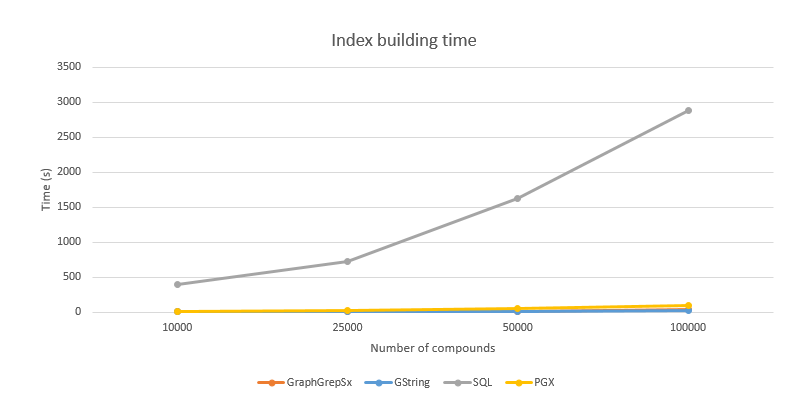
\includegraphics[width=1\textwidth]{../img/indexBuildingTime.png}
	\caption{Index building time}
	\label{fig:indextime}
\end{figure}

\begin{figure}[h]
	\centering
	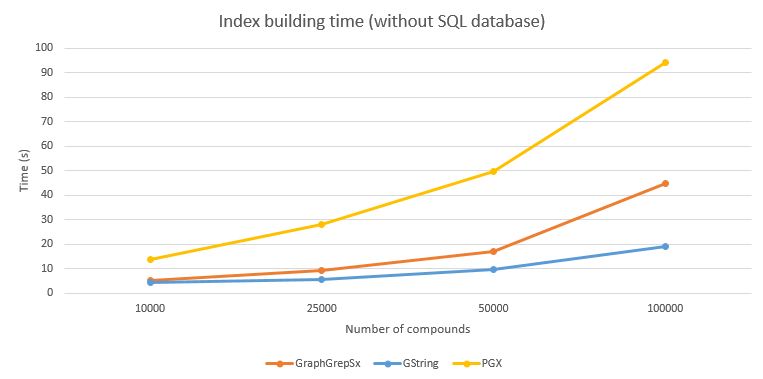
\includegraphics[width=1\textwidth]{../img/indexBuildingTimeNoSQL.png}
	\caption{Index building time without SQL database}
	\label{fig:indextimenosql}
\end{figure}

We may see that it is significantly slower to create the database from scratch than create just an index as it is in case of \textit{GraphGrepSX} and \textit{GString}. The results of database methods are quite convincing - SQL database creation time is 50 times slower compared to PGX. This is quite an expected result since PGX does work only in memory contrary to the SQL database which writes all the data to the disk.\\

In other two methods the difference is not so significant. \textit{GraphGrepSX} is two times slower than \textit{GString}. There might be two reasons for this observation. The first one is that for \textit{GString} we have used smaller parameter $l$ compared to \textit{GraphGrepSX}. The other explanation might be that it is worth to spend some time in condensation process, because it significantly reduces the number of distinct paths in the graph and therefore it makes the index building process faster.\\

We are not presenting the results for \textit{GIRAS}. The reason is that we were not able to get the results in a reasonable time. Even for 10 000 compounds we did not get the built index even after two days of computation. The reason is that the data set contains small structures which are substructures of many others and therefore there are not present any rare subgraphs.\\

After two days of computation for 10 000 compounds we stopped at the moment where we were missing indexing of 39 compounds and the currently searched support level was 600. In other words, these 39 compounds do not contain any subgraph (of maximal size of 8 vertices) which is rare enough to be a part of less than or equal to 600 compounds in the data set.\\

Just for verification, we tested \textit{GIRAS} on small datasets (hundreds of compounds) and the computation has finished in a reasonable time (several hours) and with expected results.\\

Because we were not able to build the \textit{GIRAS} index for our data set, we do not present the results of other metrics for this method since we had no way to measure them.

\section{Index and Data Size}
Since it is tricky to measure just the index size (and in a graph database this term does not even make sense) we have decided to measure the whole amount of memory needed for a particular method.\\

In case of \textit{GraphGrepSX} and \textit{GString} it is the memory used by the running process after the index is built and after triggered garbage collection.\\

In case of the SQL database we are querying the size of the index structure and \textbf{BONDS} table itself. The query looks as following:\\

\noindent\textbf{SELECT sum(bytes)/1024/1024 as "SIZE in MB"}\\
\phantom{x}\hspace{3ex} \textbf{FROM dba\textunderscore segments}\\
\phantom{x}\hspace{3ex} \textbf{WHERE segment\textunderscore name='BONDS/INDEX\textunderscore NAME'}\\

In case of graph database we use the \textit{getMemoryMb} method which is offered by the Java API of PGX graph representation.\\

The results are provided in Figure \ref{fig:indexsize}. What we found as an interesting observation is the size of the \textit{GString}'s index. After we saw these numbers we started to investigate what is the reason. It turned out that the premise that using the condensed graph to reduce the number od different paths is not valid. We have found out that the built index on the tested database contains more than one a half million nodes in the \textit{GString} index tree. The root node itself has almost 150 children, i.e. there are almost 150 different node types. This is a huge number compared to \textit{GraphGrepSX} which contains only 21 vertex node types.\\

\begin{figure}[h]
	\centering
	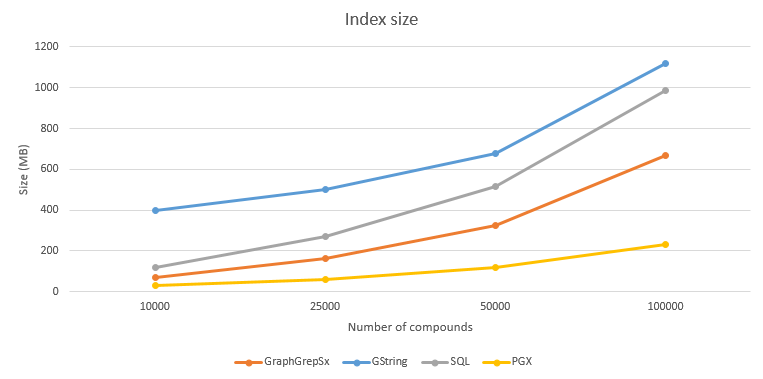
\includegraphics[width=1\textwidth]{../img/indexSize.png}
	\caption{Index size}
	\label{fig:indexsize}
\end{figure}

Other results are quite expected. The reason why PGX data representation is significantly smaller compared to SQL database is that PGX does not build any indices. The amount of memory consumed by SQL table representation (without the indices) is about the same as for PGX.

\section{Candidate Set Creation Time}
This metric is meaningful only for \textit{GraphGrepSX} and \textit{GString}. As we described in Chapter \ref{experimental}, the candidate set concept is not applicable to SQL and graph databases.\\

By candidate set creation we mean the time difference between the time when a query is executed and the time when we finish the index utilization for the particular query.\\

The results are provided in Figure \ref{fig:candidateset}. We can see that \textit{GString} is significantly slower compared to \textit{GraphGrepSX}. This is most probably because of the significantly bigger index size.\\

\begin{figure}[h]
	\centering
	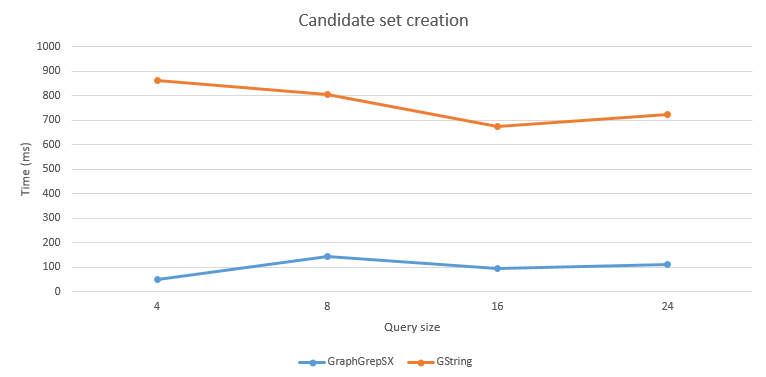
\includegraphics[width=1\textwidth]{../img/candidateSet.png}
	\caption{Candidate set creation time}
	\label{fig:candidateset}
\end{figure}

The other interesting fact for \textit{GString} is that due to the "stars versus paths" issue described in Section \ref{gstring} it is almost impossible to get meaningful results for large queries and therefore the candidate sets are cut down to almost empty sets.

\section{Verification Time}

Verification time does have two different meanings in this context. For methods where we create the candidate set, we understand verification time as time needed to verify the candidate set.\\

In case of SQL and graph databases, where we do not work with the candidate set concept, we understand verification time as the time needed for executing the query since we need to verify every single record in the database.\\

The results are provided in Figure \ref{fig:verification} in which we can observe several interesting outcomes.\\

\begin{figure}[h]
	\centering
	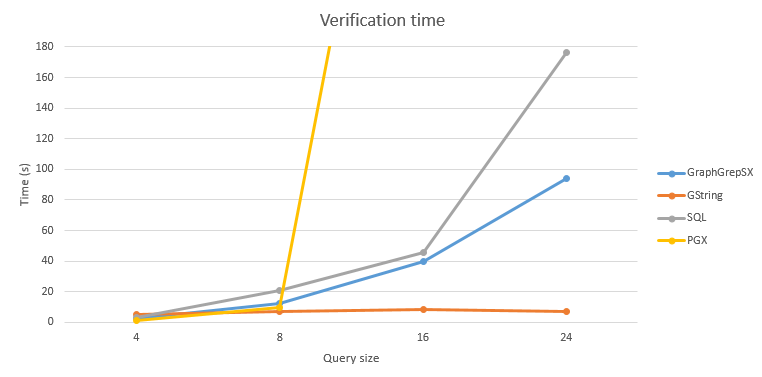
\includegraphics[width=1\textwidth]{../img/verification.png}
	\caption{Verification time}
	\label{fig:verification}
\end{figure}

At first, we can be surprised by very low numbers for verification time in case of \textit{GString}. This is caused by a significantly smaller candidate set compared to \textit{GraphGrepSX}. On the other hand, the candidate set is not smaller because of better pruning ability of \textit{GString} index, but because of the fact that \textit{GString} invalidates even the results which are valid for other methods. This was described in detail in Section \ref{gstring}.\\

The other interesting observation are the values for PGX. Although, the values for queries of sizes 4 and 8 are very good (even better than for \textit{GraphGrepSX} which is indexed) we have found out that for queries with the size bigger than 14 it is barely usable.\\

Also, we have tried to test it even on database with 1 graph with 2 vertices and 1 edge between them. We would expect that any query will be executed quickly because there is not much to compute. However, we have found that even on this small graph, big queries are very slow and the complexity grows exponentially, while query with 12 vertices took 46 seconds and query with 14 vertices took 50 minutes. Even after 3 hours of computation we were not able to get results for query with 16 vertices.\\

It seems that PGX spends a lot of time on PGQL query parsing and on creation of execution plan. We were unsure whether we did anything wrong. Luckily, the author of this thesis consulted this issue with a member of the Oracle PGX team, who confirmed that the query structure is correct and that it takes an enormous time even on Oracle internal infrastructure. We may then doubt how valid results are described in presentation \cite{pgx-neo4j} where very promising numbers even for large queries are presented.

\section{Hit Ratio of Candidate Set}
This section is only applicable for methods which create the candidate set. The metric is defined as a ratio between the candidate set size and the result set size. It measures the quality of the index, i.e. the higher the ratio is, the better results are obtained from the index.\\

The results are available in Figure \ref{fig:hitratio}. We can see that for \textit{GraphGrepSX} the efficiency of its index decreases with the query size. This is natural since the \textit{GraphGrepSX}'s index describes only paths of length up to 6. Therefore, it is expectable that with growing size of query, the accuracy will decrease, since the indexed paths cover a smaller portion of the query.\\

\begin{figure}[h]
	\centering
	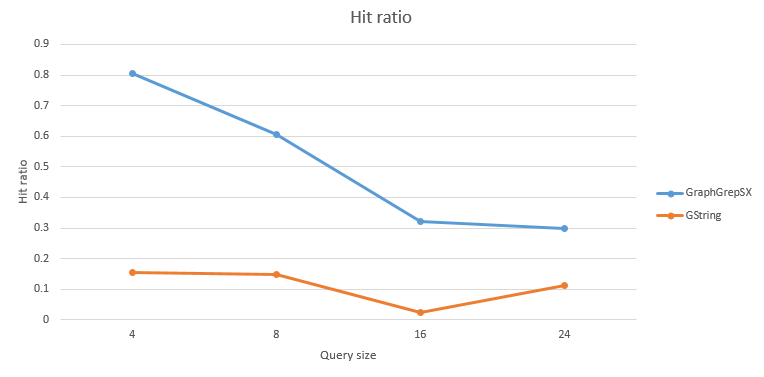
\includegraphics[width=1\textwidth]{../img/hitRatio.png}
	\caption{Candidate set hit ratio}
	\label{fig:hitratio}
\end{figure}

On the other hand, even queries of size 24 are not big enough to overflow the capacity of \textit{GString}. The condensed graph does not contain paths longer than 5 in these cases and therefore we would expect more or less constant hit ratio for all query sizes which matches the actual results. However, we can see that the hit ratio is significantly smaller compared to \textit{GraphGrepSX}.

\section{Query Execution Time}
In this section we describe the time results for the whole query process. It can be defined as a sum of the candidate set creation time and verification time. Note that in case of SQL and graph databases this is equal to the verification time. For the end user, this is probably the most crucial metric.\\

The results are provided in Figure \ref{fig:querytime}. The first thing we can observe is that this graph is not much different from the one in Figure \ref{fig:verification}. In other words, the time for obtaining a candidate set plays only very minor role in the total query time.\\

\begin{figure}[h]
	\centering
	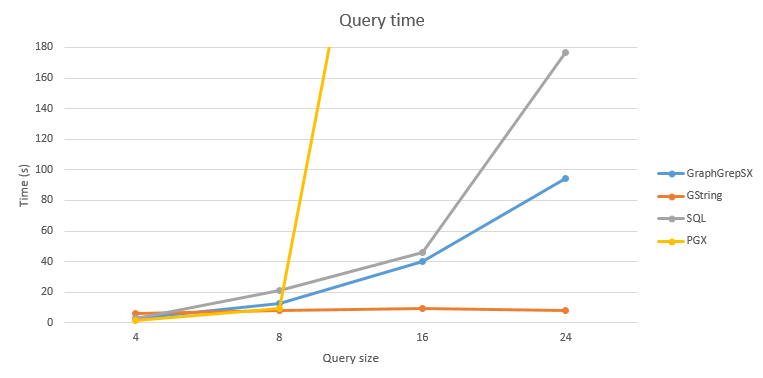
\includegraphics[width=1\textwidth]{../img/queryTime.png}
	\caption{Query time}
	\label{fig:querytime}
\end{figure}

The very good performance of \textit{GString} is a result of the fact that the result set is smaller compared to other methods. This might be confusing and a user of such method has to be aware of its limitations. On the other hand, if the user knows what are the \textit{GString} restrictions, it may be a very efficient way of querying.\\

In case of small queries, the best choice seems to be PGX. The implementation is very straight-forward and most of the work is very intuitive. Also, the implementation of PGX handler is very easily improvable to work with even much bigger data sets which cannot fit into the memory.\\

In case of the SQL database, we are quite surprised that it is a viable solution. The difference in performance times to other methods is not that significant as we would expect. Also, SQL solution is the only one which does not have to fit into memory as it is.\\

Although all other methods have their own benefits, \textit{GraphGrepSX} seems to be an overall winner. It is quite simple to implement, it has the best overall performance and reasonable index size as well as its build time.

\section{Hypotheses Results}
In this section we summarize the results of the hypotheses formulated in Section \ref{hypotheses} in Table \ref{hypothesisresults}.

\begin{table}[h]
	\centering
	\renewcommand{\arraystretch}{2.5}
	\setlength{\arrayrulewidth}{0.5mm
	}
	\begin{tabular}[h!]{|p{2cm}|p{2cm}|p{9cm}|}
		\hline
		\rowcolor{lightgray}
		Hypothesis & Result & Comments\\ \hline
		H1.1 & False & Index of \textit{GString} is significantly larger. The number of distinct nodes in case of \textit{GString} is much bigger compared to \textit{GraphGrapSX} on a real-world data set.\\ \hline
		H1.2 & Uncertain & The performance of \textit{GString} is indeed better compared to \textit{GraphGrepSX}. On the other hand, the main reason is a smaller answer set because the rules for candidate set creation are too restrictive in some cases.\\ \hline
		H2.1 & Cannot be verified & We were not able to build the \textit{GIRAS} index in a reasonable time.\\ \hline
		H2.2 & True & We were not able to build the \textit{GIRAS} index in a reasonable time even for the one tenth of the tested data set size.\\ \hline
		H3.1 & True & In general, both \textit{GraphGrepSX} and \textit{GString} perform better than SQL and PGX approaches. On the other hand, for small queries, the PGX is slightly faster. Moreover, in case of the SQL database we did expect much worse results.\\ \hline
		H3.2 & Uncertain & The hypothesis is definitely valid for small queries, in which case the performance difference is enormous. On the other hand, for larger queries PGX starts to be barely usable due to the issues with PGQL query parsing.\\ \hline
	\end{tabular}
	\caption{Hypotheses results}
	\label{hypothesisresults}
\end{table}

\chapter*{Conclusion}
\addcontentsline{toc}{chapter}{Conclusion}

In this thesis we have explored the current research about the subgraph querying of chemical databases. We have identified the most popular and the most performing indexing techniques for such purpose.\\

We have identified three indexing algorithms - \textit{GraphGrepSX}, \textit{GString} and \textit{GIRAS} - which were not compared, yet, in any related paper and which won the performance tests in the benchmarks presented as a part of the papers which describes such algorithms. We have implemented two of these algorithms - \textit{GraphGrepSX} and \textit{GString} - and we have obtained the \textit{GIRAS} source code from its author.\\

We have created a benchmark of the mentioned indexing methods which uses a data set of 100 000 chemical compounds. In this benchmark we measure the index size and its creation time, efficiency of the index and the total time needed for queries of various sizes.\\

We have also implemented a framework for testing the SQL and PGX\linebreak databases on the same data set to compare the graph oriented indexing methods to the solutions which are designed to store and query generic data.\\

We have found many of the results of related papers not completely valid. We have found out that \textit{GIRAS} does not provide complete indexing and therefore we can identify a lot of queries with invalid results. Also, we have found out that this method is barely usable on large real-world data sets since the time needed for index to be built is enormous.\\

For \textit{GString}, we have found out that its method for condensing the graph size is very efficient in the matter of acceleration the index building process, on the other hand, it omits a lot of valid results since the query graph's condensed graph does not have to match the condensed graph of actual compound which does contain the graph query as its subgraph.\\

Also, one of the main reasons of graph condensation in \textit{GString} is to make the index smaller compared to \textit{GraphGrepSX}. We have proved that on real-world data set this is not a valid presumption because the size of the vertex label set on such database is significantly smaller compared to the size of distinct vertex labels on condensed graphs where we introduce a new label for each distinct size of path, cycle or star respectively.\\

We have found PGX as a viable and very well performing solution for small queries. On the other hand, the performance for larger queries is getting worse exponentially and it becomes barely usable even for queries of size 16. We have reported this issue to Oracle. This result seems to be very close the observation made by Hoksza et al. in \cite{Hoksza}\\

In case of other two methods - SQL database and \textit{GraphGrepSX} - we have been surprised by their performance. Even though, SQL database has been the only technique which does use disk for storing the data, its performance is not bad at all and it seems to be a viable solution for data sets which cannot fit into the memory.\\

Although \textit{GraphGrepSX} is much simpler indexing technique compared to the other described ones, we have identified it as best performing. It is not anyhow customized to be used for chemical databases and can be utilized for any data which can be described by graphs.

\section*{Future Work}
\addcontentsline{toc}{section}{Future Work}
All described indexing techniques do work only in memory. This is a significant issue for big databases. It might be an interesting research to find out the possibilities of improving the described methods to store the indices on the disk. Or even better, divide the chemical compounds into some classes and store these separately in different indices.\\

The other interesting research might be to compare our benchmark results to the performance of the commercially used solutions which we have described in the Analysis Section of this thesis. 

 


%%% Bibliography
%%% Bibliography (literature used as a source)
%%%
%%% We employ bibTeX to construct the bibliography. It processes
%%% citations in the text (e.g., the \cite{...} macro) and looks up
%%% relevant entries in the bibliography.bib file.
%%%
%%% The \bibliographystyle command selects, which style will be used
%%% for references from the text. The argument in curly brackets is
%%% the name of the corresponding style file (*.bst). Both styles
%%% mentioned in this template are included in LaTeX distributions.

% \bibliographystyle{plainnat}    %% Author (year)
\bibliographystyle{unsrt}     %% [number]

\renewcommand{\bibname}{Bibliography}

%%% Generate the bibliography. Beware that if you cited no works,
%%% the empty list will be omitted completely.

\bibliography{bibliography}

%%% If case you prefer to write the bibliography manually (without bibTeX),
%%% you can use the following. Please follow the ISO 690 standard and
%%% citation conventions of your field of research.

% \begin{thebibliography}{99}
%
% \bibitem{lamport94}
%   {\sc Lamport,} Leslie.
%   \emph{\LaTeX: A Document Preparation System}.
%   2nd edition.
%   Massachusetts: Addison Wesley, 1994.
%   ISBN 0-201-52983-1.
%
% \end{thebibliography}


%%% Figures used in the thesis (consider if this is needed)
\listoffigures

%%% Tables used in the thesis (consider if this is needed)
%%% In mathematical theses, it could be better to move the list of tables to the beginning of the thesis.
\listoftables

%%% Abbreviations used in the thesis, if any, including their explanation
%%% In mathematical theses, it could be better to move the list of abbreviations to the beginning of the thesis.
\chapwithtoc{List of Abbreviations}

%%% Attachments to the master thesis, if any. Each attachment must be
%%% referred to at least once from the text of the thesis. Attachments
%%% are numbered.
%%%
%%% The printed version should preferably contain attachments, which can be
%%% read (additional tables and charts, supplementary text, examples of
%%% program output, etc.). The electronic version is more suited for attachments
%%% which will likely be used in an electronic form rather than read (program
%%% source code, data files, interactive charts, etc.). Electronic attachments
%%% should be uploaded to SIS and optionally also included in the thesis on a~CD/DVD.
\chapwithtoc{Attachments}

\openright
\end{document}
